\documentclass[border=4pt]{standalone}
% Shared style for every diagram. Colour-blind-safe palette (Okabe-Ito).
\usepackage[T1]{fontenc}
\usepackage{helvet}
\renewcommand{\familydefault}{\sfdefault}
\usepackage{tikz}
\usetikzlibrary{arrows.meta,positioning,fit,backgrounds,calc,shapes.geometric,decorations.pathreplacing}
\definecolor{cblue}{HTML}{0072B2}
\definecolor{corange}{HTML}{E69F00}
\definecolor{cgreen}{HTML}{009E73}
\definecolor{cred}{HTML}{D55E00}
\definecolor{cpurple}{HTML}{CC79A7}
\definecolor{cgrey}{HTML}{6B7280}
\definecolor{csky}{HTML}{56B4E9}
\tikzset{
  >={Stealth[length=2.2mm]},
  box/.style={draw, rounded corners=3pt, align=center, minimum height=11mm, minimum width=22mm, font=\small, line width=0.7pt},
  real/.style={box, draw=cblue, fill=cblue!8},
  sim/.style={box, draw=corange, fill=corange!12},
  future/.style={box, draw=cgrey, dashed, fill=white},
  flow/.style={->, line width=0.8pt, draw=black!75},
  dflow/.style={->, line width=0.8pt, dashed, draw=cgrey},
  lbl/.style={font=\scriptsize, text=black!70},
  group/.style={draw=black!25, rounded corners=6pt, inner sep=6pt},
}

\begin{document}
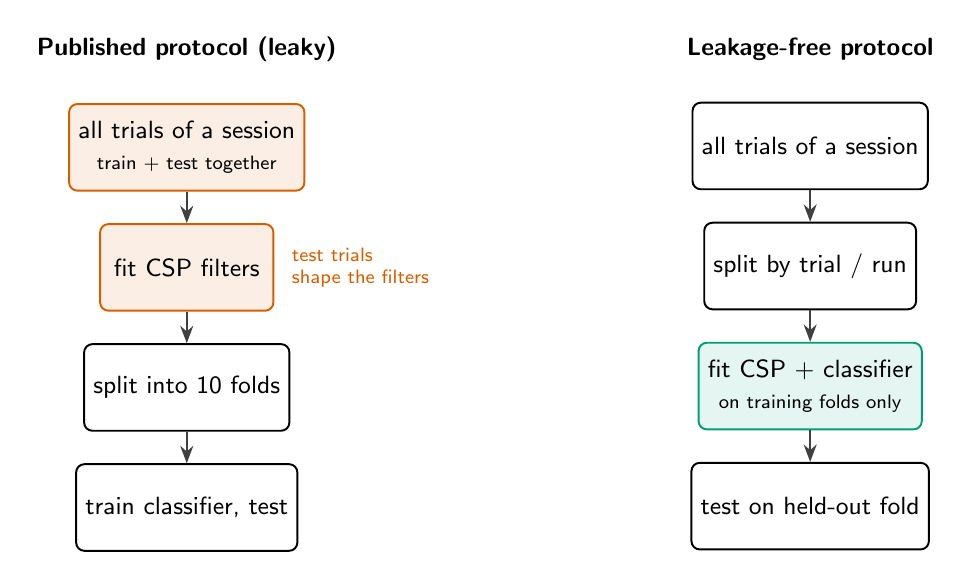
\begin{tikzpicture}[node distance=4mm]
  % published protocol
  \node[font=\small\bfseries] (t1) {Published protocol (leaky)};
  \node[box, below=of t1, draw=cred, fill=cred!10] (a1) {all trials of a session\\\scriptsize train + test together};
  \node[box, below=of a1, draw=cred, fill=cred!10] (a2) {fit CSP filters};
  \node[box, below=of a2] (a3) {split into 10 folds};
  \node[box, below=of a3] (a4) {train classifier, test};
  \foreach \a/\b in {a1/a2, a2/a3, a3/a4} \draw[flow] (\a) -- (\b);
  \node[lbl, right=1mm of a2, text=cred, align=left] {test trials\\shape the filters};
  % leak-free
  \node[font=\small\bfseries, right=42mm of t1] (t2) {Leakage-free protocol};
  \node[box, below=of t2] (b1) {all trials of a session};
  \node[box, below=of b1] (b2) {split by trial / run};
  \node[box, below=of b2, draw=cgreen, fill=cgreen!10] (b3) {fit CSP + classifier\\\scriptsize on training folds only};
  \node[box, below=of b3] (b4) {test on held-out fold};
  \foreach \a/\b in {b1/b2, b2/b3, b3/b4} \draw[flow] (\a) -- (\b);
\end{tikzpicture}
\end{document}
